% Pursuing Stacks (cotes 134-2 to 134-8): archive cote 134-4, site page 1 (PDF page 2), typescript page 89.
% typescript. Draft compared: ps3.tex:1-59.
% AI-transcribed by Claude Opus 5.5 (claude-opus-5-5, adaptive thinking, effort high), Message Batches API, batch ps1 (msgbatch_01Rv5hCaNTtUt4JHx1yqoHPL), 2026-11-12; image review recorded in records/CHECK_DECISIONS_134_3_4.tsv.
\scanpage{134-4/1}
\margin{\diagram{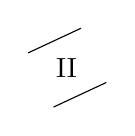
\begin{tikzpicture}[rotate=25]\node[inner sep=1pt] (n) {II};\draw (-.36,.38)--(.38,.38);\draw (-.36,-.38)--(.38,-.38);\end{tikzpicture}}}
\mspage{(89)}
27.3.

45.    The review yesterday of the various ``test notions'',  turning
around test \over[typed]{c}{c}ategories and test functors,  turned out a lot longer than
expected,  so much so \deleted{as} to \inserted{have me} get a little weary by the end  -  it was clear
though that this ``travail d'intendance'' was necessary,  not only not to
get lost in a morass of closely related and yet definitely distinct noti-%
ons,  but also to gain perspective and a better feeling of the formal struc%
ture of the whole set-up.  As has been the case so often, \over{a}{d}uring this
\deleted{ungratifying} \inserted{very} work of ``grinding through'',  there has appeared \xout{again} this
caracteristic feeling of getting close to something ``burning'' again, some-%
thing very simple-minded surely which has kept showing up gradually and
more and more on all odds and ends,  and \inserted[typed]{which} still is escaping,  still elusive\hand{.}
T$\overset{\hand{\unsure{\wedge}}}{\mathrm{h}}$ere is an impressive bunch of things \deleted{though} which are demanding pressing%
ly  more or less immediate investigation  -  still I can't help,  I'll
have to try and pin down some way or other this \hand{``}burning spot\hand{''}.

T\over[typed]{H}{h}ere seem to be recurring striking features of the modelizers met
with so far  -  namely essentially (Cat) and the elementary modelizers $A^{\hand{\wedge}}$
and possibly their ``weak'' variants.  I\over[typed]{N}{n} all of them,  there is a very
strong interplay between the following notions,  which seem to be the
basic ones and \over{\unsure{m}}{m}ore or less determine each other mutually:  \uline{weak equiva-}%
\uline{lences} (which define the modelizing structure of the given modelizer M),
\uline{aspheric objects}  (namely such that  $x \hand{\to} e_M$ is a weak equivalence),
\uline{homotopy intervals}  $(I,\hand{\delta}_0,\hand{\delta}_1)$,  and last not least,  the notion of a test
functor  $A \hand{\longrightarrow} M$ ,  where A is a test category (or more generally weak
test functors of weak test categories into M).  The latter so far have
been defined only when M = (Cat),  and initially they were viewed \xout{rather}
as being mainly  more handy substitu\over{\unsure{t}}{t}\over{e}{e}\over{s}{s} to \xout{functors} $j_A$\hand{,} for getting a
model-preserving functor (Cat)$\hand{\to}$ $A^{\hand{\wedge}}$ quasi-inverse to the all-important
\xout{functor} model-preserving functor \xout{\illegible{1}}  $i_A : A^{\hand{\wedge}}\hand{\to}$(Cat) ,  $F \hand{\mapsto} A_{\hand{/}F}$ .  I sus-%
pect however that their role is \inserted[typed]{a} considerably more basic one than just
computational convenience  -  and this reminds me of the analoguous fee-%
ling I had,  when first contemplating using such a thing as (by then still
vaguely conceived) ``test categories'',  for investigating ways of putting
modelizing structures on categories M such as categories of algebraic
structures of some kind or \xout{r}\over[typed]{\unsure{a}}{o}ther. (Cf. notes of march 7,  and more speci-%
fically par. 26  -  this was the very day,  by the way,  I first had th\over{e}{i}\over{s}{s}
feeling of being ``burning'' ...)

\margin{1}
